\documentclass[xcolor=table]{beamer}

\usetheme[secheader,compress]{Madrid} %Primary theme

\usepackage{verbatim}
\usepackage{graphicx}
\usepackage{hyperref}
\usepackage{enumerate}

%% UTM Colors
\definecolor{UTMblue}{rgb}{0.043137, 0.137254, 0.254901}
\definecolor{UTMorange}{rgb}{1.0, 0.509803, 0}

\setbeamercolor{palette primary}{bg=UTMblue,fg=white}
\setbeamercolor{palette secondary}{bg=UTMblue,fg=white}
\setbeamercolor{palette tertiary}{bg=UTMblue,fg=white}
\setbeamercolor{palette quaternary}{bg=UTMblue,fg=white}
\setbeamercolor{structure}{fg=UTMblue} % itemize, enumerate, etc
\setbeamercolor{section in toc}{fg=UTMblue} % TOC sections
\setbeamercolor{title}{fg=UTMorange}

\setbeamercolor{subsection in head/foot}{bg=UTMorange,fg=white}

%%%%%%%%%%% BEGIN MACROS %%%%%%%%%%%%%%%%%%
% frameT: Frame with title
\newcommand{\frameT}[2]{\frame{\frametitle{#1} #2}}

% frameF: Fragile frame with title
\newcommand{\frameF}[2]{
  \begin{frame}[fragile]
    \frametitle{#1}
    #2
  \end{frame}
}

% frameTop: Frame aligned t the top
\newcommand{\frameTop}[2]{\frame[t]{\frametitle{#1} #2}}


\newcommand{\tab}{\hspace{1cm}}

\newcommand{\spaceor}{\hspace{5pt} \textbf{or} \hspace{5pt}}

%%%%%%%%%%% END MACROS %%%%%%%%%%%%%%%%%%%%



\begin{document}

\title{ParkSense}

\author{Aaron Alden, Spencer Karpati, Zachary Rose}
\institute{UT-Martin}
\date{\today}

%%%%%%%%%%% BEGIN TITLE %%%%%%%%%%%%%%%%%%
\frame{\titlepage}

 %\section{Outline}
%%%%%%%%%%%% END TITLE  %%%%%%%%%%%%%%%%%%


\section{Introduction}
\frameT{Motivation} {
   \begin{figure}[ht]
   \hspace{-2.0cm}\begin{minipage}[c]{0.5\linewidth}
   Background
   \smallskip
  \begin{enumerate}
  \item Parking Shortage%
      \bigskip
    \item Computer Vision%
     \bigskip
  \end{enumerate}
   \end{minipage}
   \hspace{-1.0cm}\begin{minipage}[c]{0.4\linewidth}
\centering
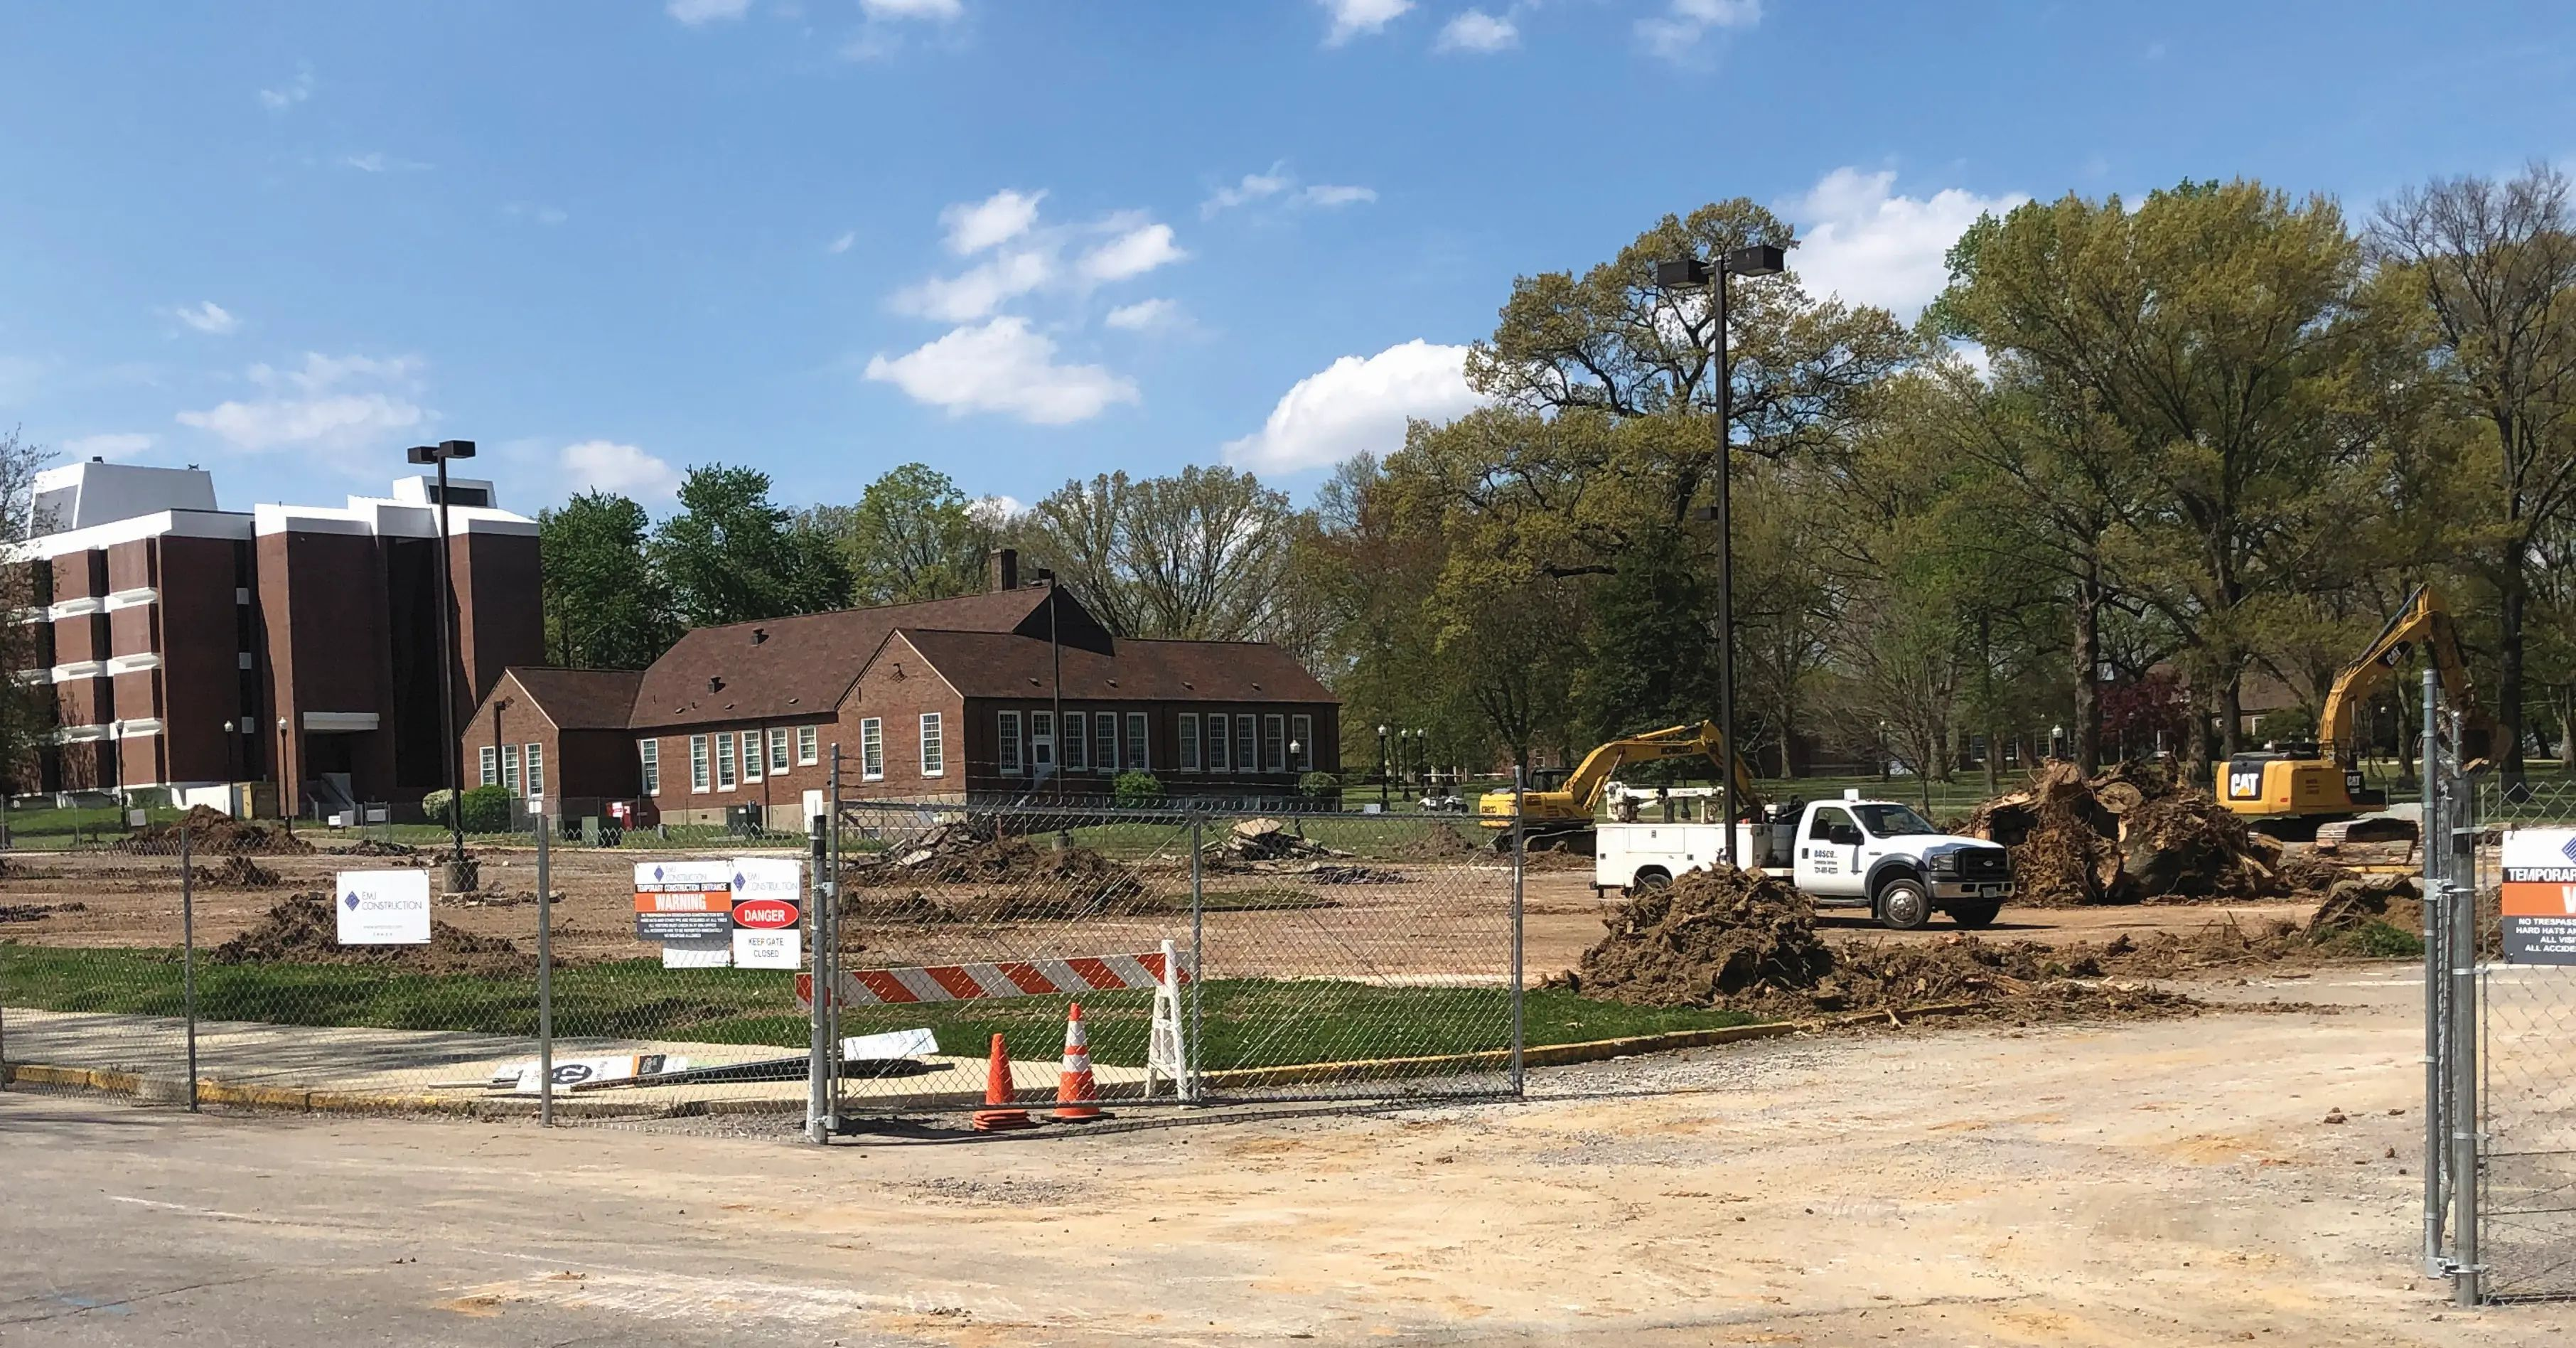
\includegraphics[width=1.3\linewidth]{figures/humanities_lot_before.jpg}
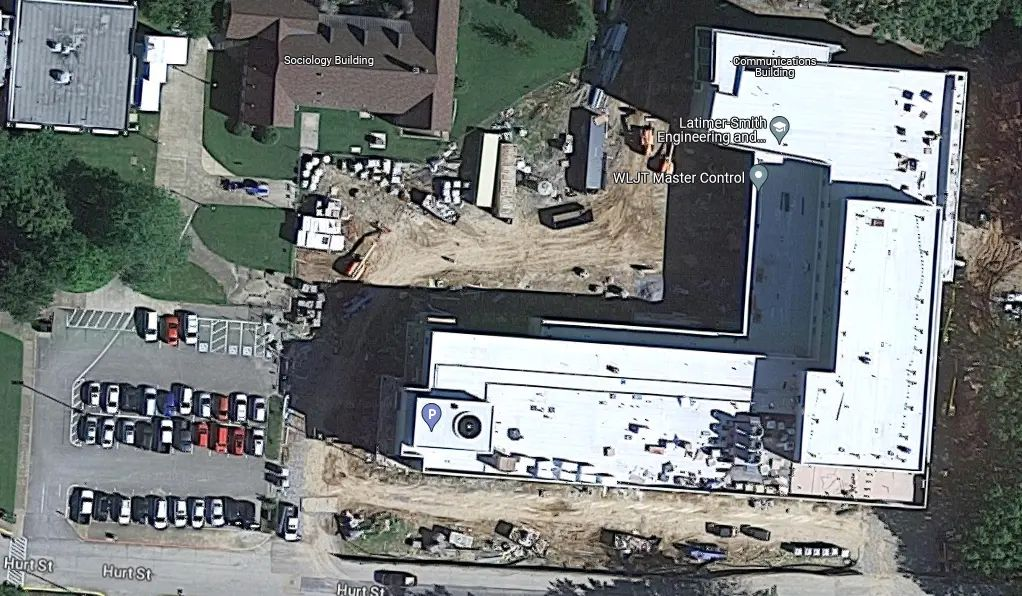
\includegraphics[width=1.3\linewidth]{figures/humanities_lot_after.jpg}
   \end{minipage}
 \end{figure}
}

%\frameT{Project Goals} {
 % Described what you are trying to accomplish, including ``stretch'' goals.
%}

%\section{Sections--a useful organizational tool.}
\section{}

\frameT{Technology}{
\begin{figure}[ht]
   \begin{minipage}[c]{0.5\linewidth}
\begin{enumerate}
    \item Computer Vision and Machine Learning
    \begin{enumerate}[(a)]
        \item OpenCV
        \bigskip
        \item Ultralytics: YOLOv8
    \end{enumerate}
    \bigskip
    \item Hardware
    \begin{enumerate}[(a)]
    % Mention portability
        \item Raspberry Pi 2 Model B
        \bigskip
        \item Raspberry Pi Camera Module
    \end{enumerate}
  \end{enumerate}
  \end{minipage}
   \hspace{0.5cm}
   \begin{minipage}[c]{0.4\linewidth}
\centering
      \vspace{0.3cm}
    
\includegraphics[width=.6\linewidth]{figures/opencv_logo.png}
       \vspace{0.5cm}
    
\includegraphics[width=0.7\linewidth]{figures/ultralytics_logo.jpg}
    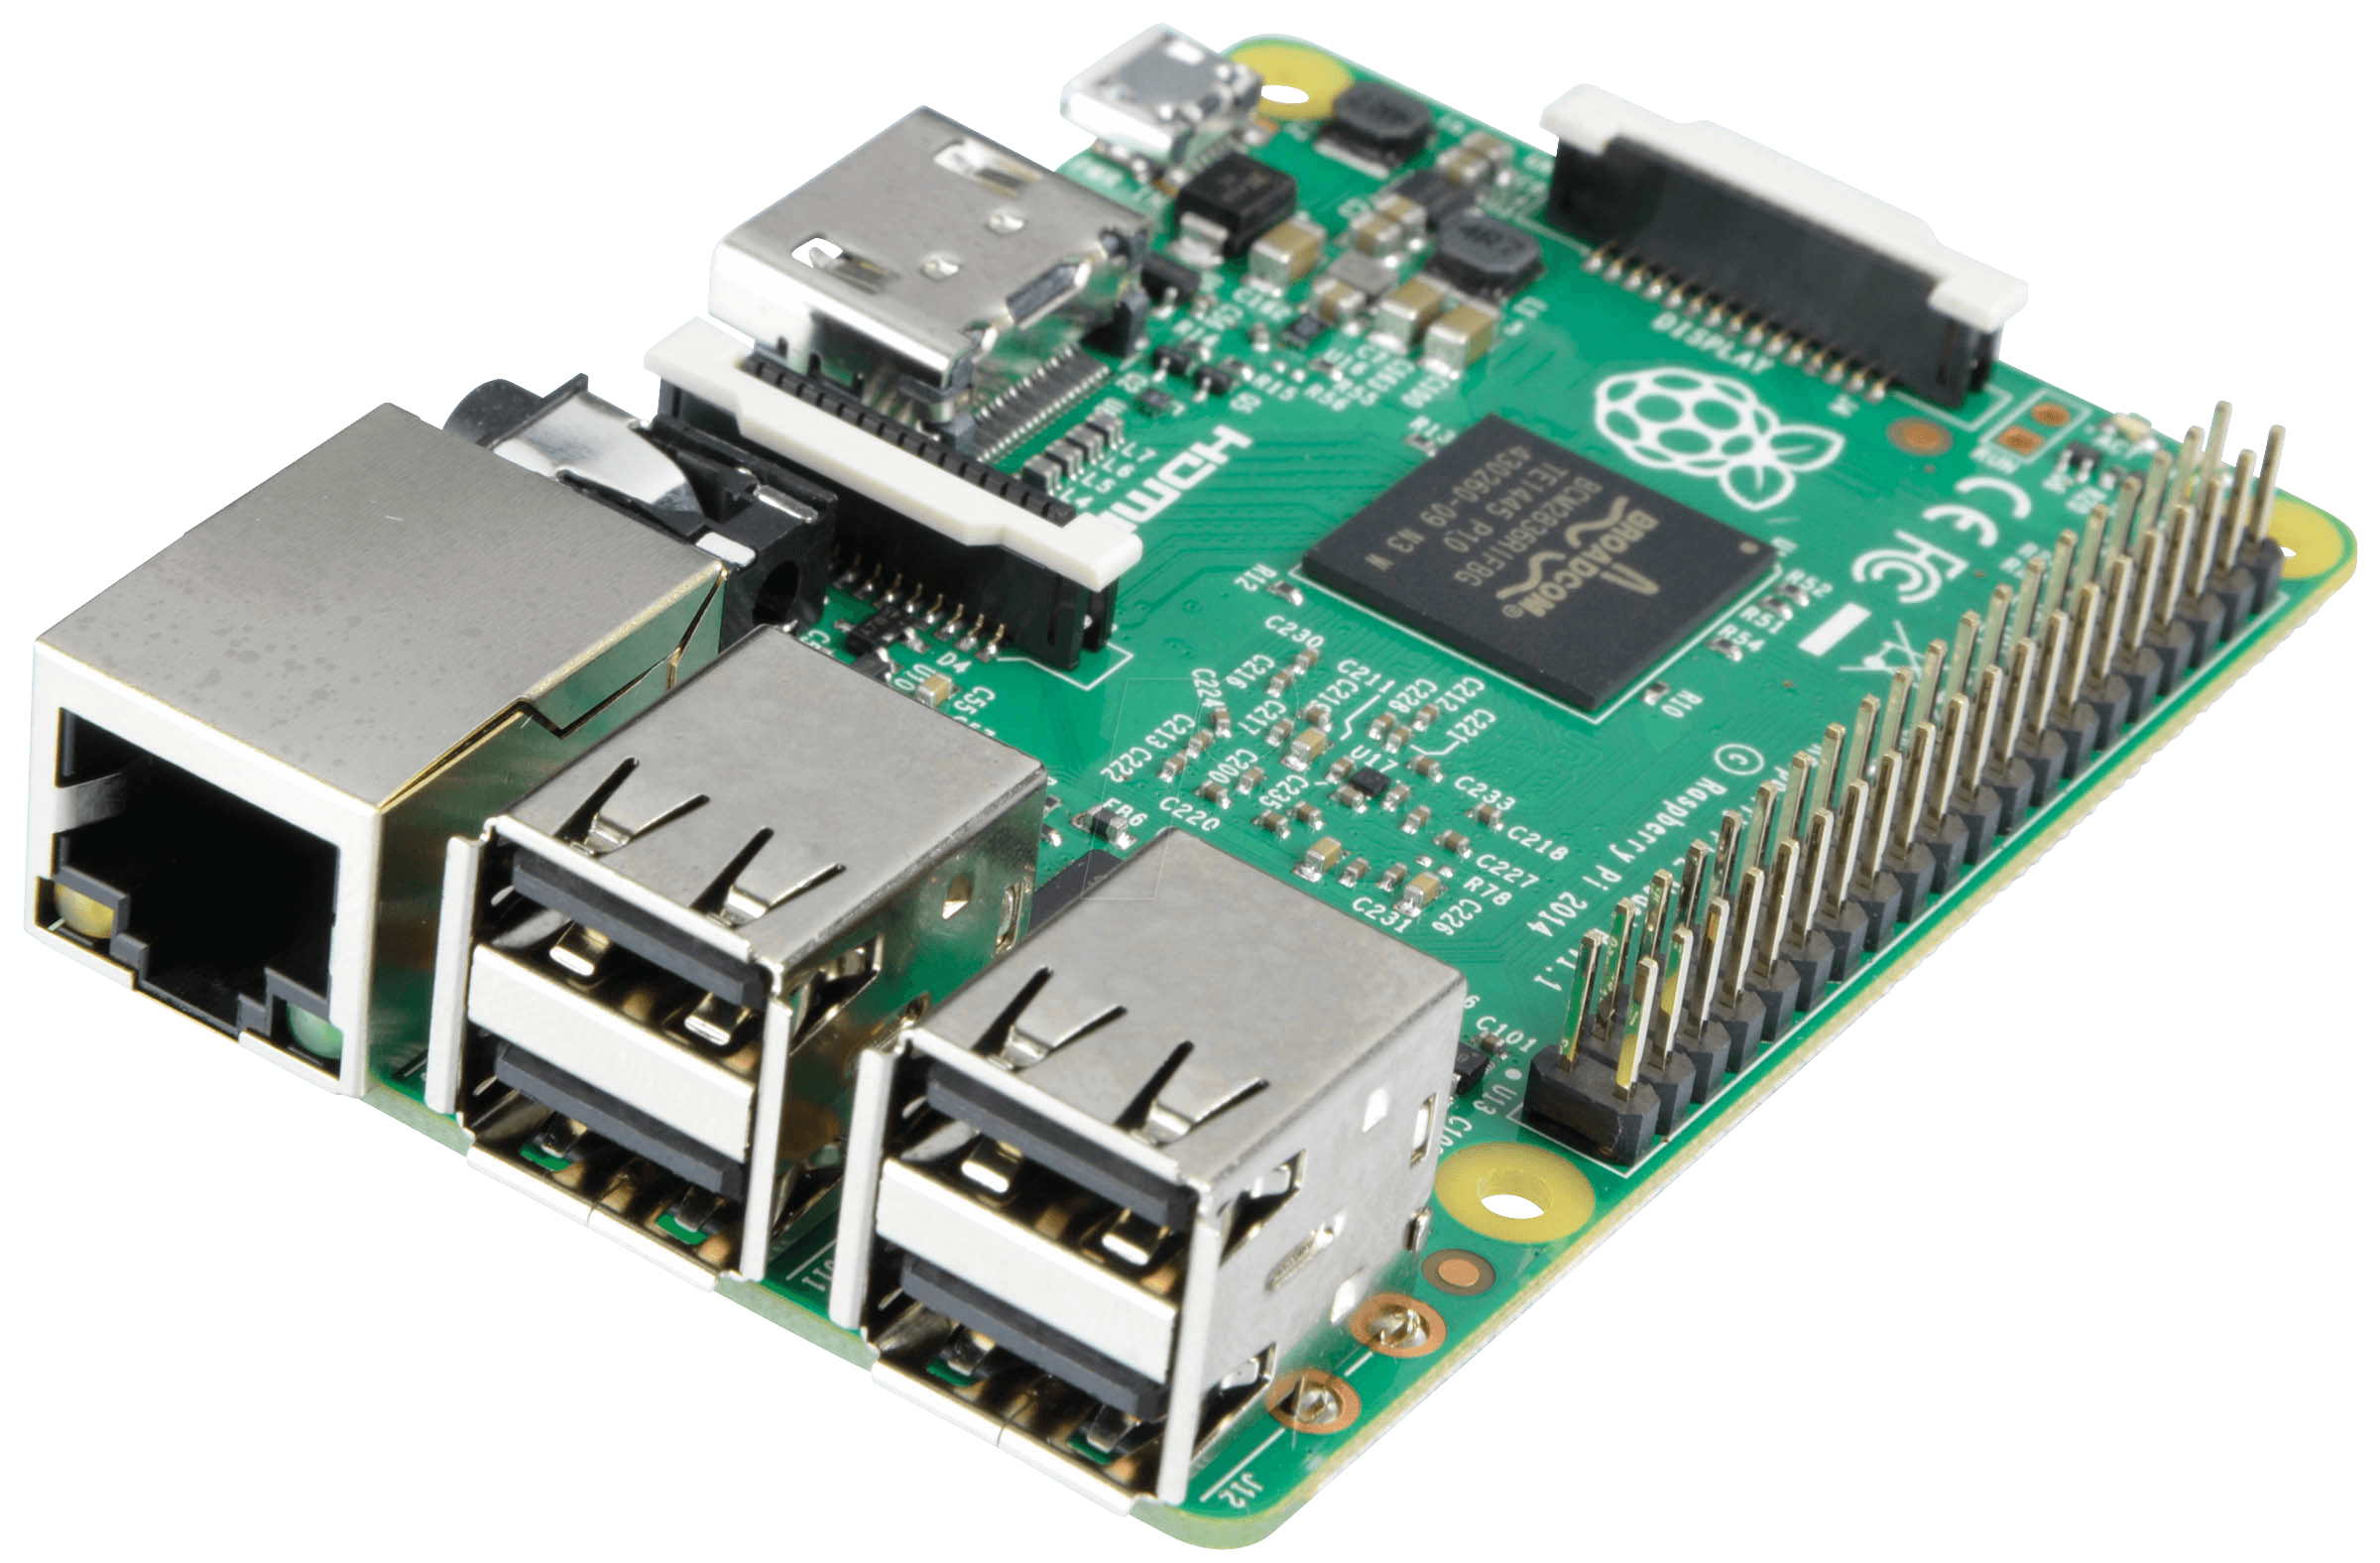
\includegraphics[width=0.5\linewidth]{figures/raspberrypi.png}
   \end{minipage}
   \end{figure}
}

\frameT{Goals}{
\begin{enumerate}
    \item Provide a web dashboard with lot information
    \begin{enumerate}[(a)]
        \item Current spot availability
        \bigskip
        \item Predictive trends
    \end{enumerate}
    \bigskip
    \item Set precedent for similar projects
    \begin{enumerate}[(a)]
        \item Training custom data sets with machine learning
        \bigskip
        \item Portable computing and networking
    \end{enumerate}
  \end{enumerate}
}

\frameT{Demonstration}{
\centering
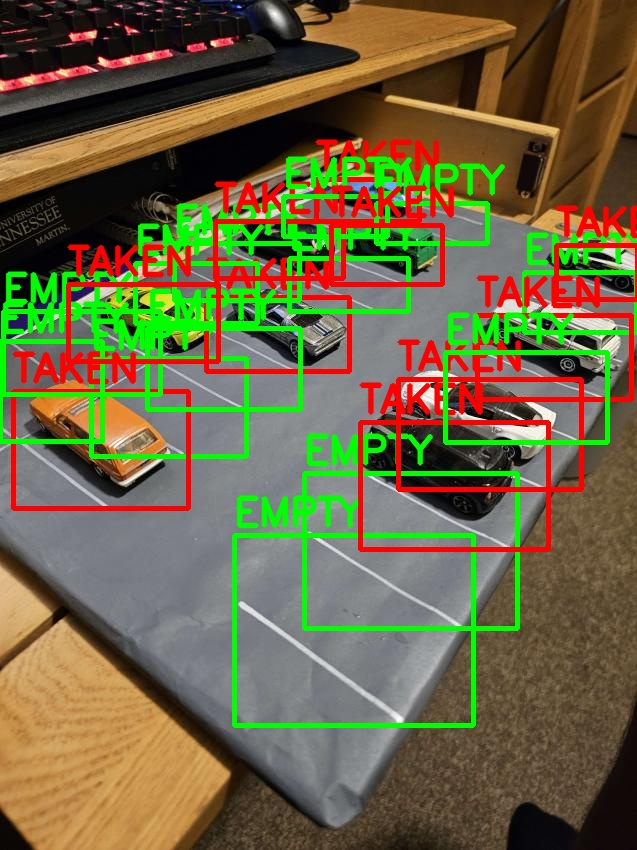
\includegraphics[width=.4\linewidth]{figures/lot_2.jpg}

\href{https://spencek7746.github.io/Senior-Design-Project}{Webpage}
}


\frameT{Challenges}{
   \begin{figure}[ht]
   \begin{minipage}[c]{0.5\linewidth}
  \begin{enumerate}
  \item Compiling on low power devices%
      \bigskip
    \item Converting camera feed to usable input%
     \bigskip
  \end{enumerate}
   \end{minipage}
   \hspace{0.5cm}
   \begin{minipage}[c]{0.4\linewidth}
\centering
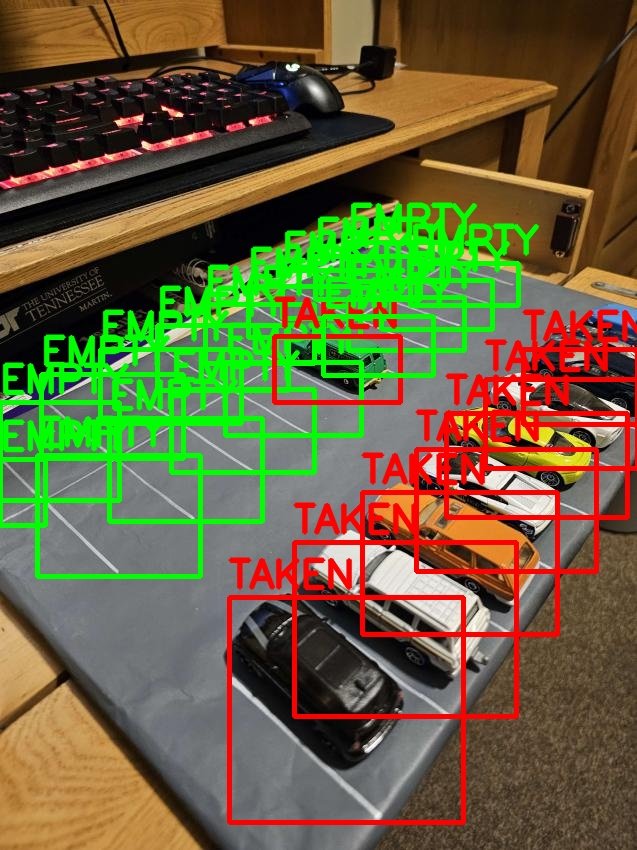
\includegraphics[width=0.9\linewidth]{figures/lot_3.jpg}
   \end{minipage}
   \end{figure}
}

\frameT{Future Work}{
\begin{enumerate}
    \item Monitor a real lot
    % \begin{enumerate}[(a)]
    %     \item OpenCV
    %     \bigskip
    %     \item Ultralytics: YOLOv8
    % \end{enumerate}
    \bigskip
    \item Push notifications
    \begin{enumerate}[(a)]
        \item Optional messages through text or email
    \end{enumerate}
    \bigskip
    \item Statistical analysis of parking trends
  \end{enumerate}

}
%\begin{frame}[fragile]
%\frametitle{Family Tree Knowledge Base}
%Facts:
%\begin{verbatim}
%Verbatim is a great way of enumerating code/algorithmic ideas.
%\end{verbatim}
%\end{frame}


%\frameT{How to include images} {
  %% \includegraphics[width=.7\linewidth]{figures/image.pdf}
%}


%\begin{frame}[fragile]
%  \frametitle{Social Network Graph}
%  \begin{figure}[ht]
%    \begin{minipage}[b]{0.53\linewidth}
%      \centering
%      Minipages are a great way to
%    \end{minipage}
%    \hspace{0.5cm}
%    \begin{minipage}[b]{0.4\linewidth}
%      \centering
%      Line up side-by-side content.

%    \end{minipage}
%  \end{figure}
  
%\end{frame}


%\frameT{Results} {
%  Describe any results of your work here.

%  \bigskip

%  Things that worked?

%  \bigskip

%  Things that didn't work?
%}

%\frameT{Conclusions} {
%  Some bullet points here to wrap things up.
%}

\frameT{Any Questions?} {
  
  \begin{center}
    Questions?
  \end{center}
  \begin{center}
    Comments?
  \end{center}

  \bigskip

  Further project/author information:
  \begin{center}
  Please see our Github repo: \href{https://github.com/Spencek7746/Senior-Design-Project}{https://github.com/Spencek7746/Senior-Design-Project}
  \end{center}
  \begin{center}
    
\includegraphics[width=4cm]{figures/6AnLddq.png}
  \end{center}
}

%\frameF{fragile test} {
%}

%% \frameF{Prolog Family Tree} {
%% \begin{verbatim}
%% hello
%% \end{verbatim}



%% }

%Empty Page
%\frameT{Frame 1}{
%}  


\end{document}
